\documentclass[a4paper]{report}
\usepackage[utf8]{inputenc}
\usepackage[T1]{fontenc}
\usepackage[english,main=french]{babel}
\usepackage[babel=true]{csquotes}
\usepackage{translator}
\usepackage{graphicx}
\usepackage{float}
\usepackage[export]{adjustbox}
\usepackage{amsmath}
\usepackage{algorithm2e}
\usepackage{hyperref}
\usepackage{listings}
\usepackage{pgfgantt}
\usepackage[toc,page]{appendix}
\usepackage[backend=biber,style=alphabetic]{biblatex}
\usepackage{glossaries}

\providetranslation[to=french]{April}{Avril}
\providetranslation[to=french]{May}{Mai}
\providetranslation[to=french]{June}{Juin}
\providetranslation[to=french]{July}{Juillet}
\providetranslation[to=french]{August}{Août}

\graphicspath{ {../images/} }
\addbibresource{refs.bib}
\nocite{*}
\RestyleAlgo{ruled}
\renewcommand{\appendixpagename}{Annexes}
\renewcommand{\appendixtocname}{Annexes}
\hypersetup{
    colorlinks=true, %colorise les liens
    breaklinks=true, %permet le retour  la ligne dans les liens trop longs
    urlcolor=blue, %couleur des hyperliens
    linkcolor=black, %couleur des liens internes
    bookmarksopen=true, %si les signets Acrobat sont crs, les afficher compltement.
}


\title{Rapport de stage}
\author{Oscar Buon}


\begin{document}


\begin{titlepage}
    \centering
    \begin{minipage}{0.45\textwidth}
        
\includegraphics[width=\textwidth]{logo_ISIMA_INP.png}
    \end{minipage}\hfill
    \begin{minipage}{0.45\textwidth}
        
\includegraphics[width=\textwidth]{logo_CERN.png}
    \end{minipage}

    \vfill

	{\Large
        Rapport d'élève ingénieur \par
        Stage de 2ème année \par
        Filière 1 : Informatique des systèmes interactifs pour l’embarqué, la robotique et le virtuel \par
    }

	\vfill

	{\huge\bfseries Speeding up LHCb software through compilation optimization \par}

	\vfill

	{\Large Présenté par : Oscar Buon \par}

	\vfill

	Responsable Entreprise : Sébastien Ponce \par
	Responsable ISIMA : Mamadou Kanté

	\vfill

	4 septembre 2023
    Stage de 5 mois

    \vfill

    Campus des Cézeaux. 1 rue de la Chebarde. TSA60125. 63178 Aubière CEDEX
\end{titlepage}


\pagenumbering{Roman}
\chapter*{Remerciements}
    J'aimerais commencer par remercier Sébastien Ponce, mon tuteur de stage sans qui mon travail au CERN n'aurait pas été possible et qui m'a aidé tout au long.

    Merci égallement à M. Mamadou Kanté, tuteur ISIMA et responsable de la fillière.

    \bigskip
    Je tiens aussi à remercier Alexandre Boyer qui m'a permis à l'occasion du forum ingénieur de trouver un stage au CERN.

    \bigskip
    Merci à Marco Clemencic qui m'a plusieurs fois aidé à résoudre certains problèmes.

    \bigskip
    Enfin je remercie Gloria Corti et Marco Cattaneo qui m'ont fait visité LHCb et DELPHI sous terre.

\tableofcontents

\listoffigures


\begin{abstract}
    Ce stage a pour objectif d'étudier l'infrastructure logicielle qui traite les données du détecteur LHCb du CERN et de mettre en place des solutions pour l'optimiser via une meilleure compilation.
    Les programmes sont principalement codés en C++ et compilés via CMake.

    Plusieurs méthodes ont été essayées.
    La première a été de fusionner les centaines de bibliothèques dynamiques en un seul exécutable.
    L'utilisation de profile-guided optimization et de link-time optimization a égallement été mise en place.

    Une amélioration d'environ $7\%$ a été obtenue avec le profile-guided optimization et le link-time optimization.

    \vfill

    Mots-clés : LHCb, Optimisation, Compilation avancée

\end{abstract}

\begin{otherlanguage}{english}
\begin{abstract}

    \vfill

    Key words : LHCb, Optimization, Advanced compilation
\end{abstract}
\end{otherlanguage}


\pagenumbering{arabic}
\chapter*{Introduction}
    LHCb est l'une des 4 principales expériences du Large Hadron Collider (LHC) du CERN.
    À l'intérieur se font plus de 30 millions de collisions par secondes, ce qui produit un flux de données d'environ $5 To/s$.
    Ces données doivent rapidemment être traitées pour reconstruire les trajectoires des particules et pour pouvoir être analysées tout autour du monde.

    L'infrastucture logicielle de traitement est principalement écrite en C++ et en Python.
    Du code est ajouté ou modifié tous les jours par plusieurs centaines de membres de la collaboration, qui représentent 83 instituts dans 19 pays en 2020.
    Cela représente des millions de lignes de codes qu'il faut maintenir et améliorer.
    Pour gérer cela, des outils modernes comme gcc, clang ou CMake sont utlisés.

    L'objectif du stage est d'abord de proposer et d'implémenter des solutions pour améliorer l'éfficacité des programmes.
    De plus, la mise en place de systèmes aidant au maintient de l'infrastrucutre peuvent être étudiés.

    D'abord sera étudier la possiblité d'utiliser des bibliothèques statiques à la place des dynamiques.
    Ensuite sera aborder la mise en place de profile-guided optimization pour la compilation des programmes.
    Aussi la mise en place d'outils permettant de mieux gérer les inclusions dans le code source sera envisagée.
    Enfin sera étudier l'impact de l'utilisation du \emph{fast math} sur la rapidité et la stabilité des programmes.

    La première parti de ce rapport est consacrée à l'étude et l'analyse des problèmes.
    La seconde explique les méthodes et solutions techniques utilisées.
    La dernière rend compte des résultats.


\chapter{Introduction}
    \section{Présentation du CERN}
        L'Organisation européenne pour la recherche nucléaire est le plus grand laboratoire d'étude de la physique des particules au monde.
        Le centre, qui a été fondé en 1954, se situe sur la frontière franco-suisse à quelques kilomètres de Genève.

        Une grande partie des recherches éffectuées au CERN utilisent différents accélérateurs de particules.
        Le principe est de faire atteindre à des particules des vitesses proches de celle de la lumière pour qu'elles acquièrent une grande énergie, puis de les faire se collisionner.
        La physique des particules prévoit l'apparition de nouvelles particules lors de ces collisions.
        Ainsi en détectant les collisions au seins de l'accélérateur et en comparant avec la théorie, on peut la valdier ou l'invalider.

        Il existe plusieurs accélérateurs et plusieurs expériences au CERN.
        Le plus grand accélérateur est le Grand collisionneur de hadrons ou Large Hadron Collider (Figure \ref{LHC}) qui a été mis en fonction en 2008 et qui a une circonférence d'environ 27 kilomètres.
        Il permet d'accélérer des protons à environ $7 Tev$.

        \begin{figure}[!htb]
            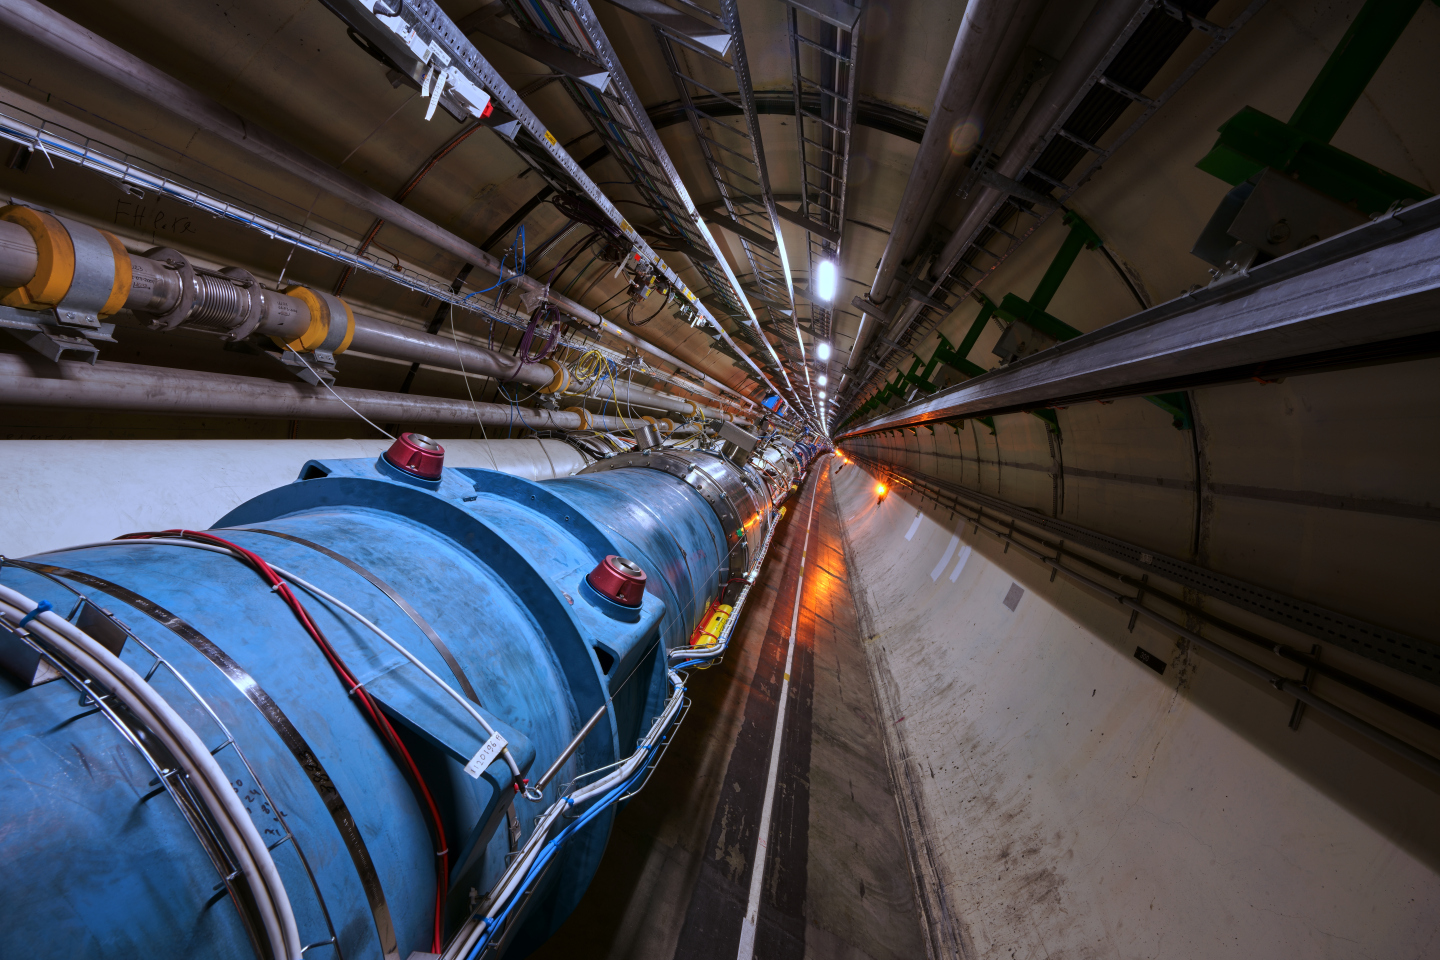
\includegraphics[width=\textwidth, center]{LHC.jpg}
            \caption{LHC}
            \label{LHC}
        \end{figure}

        Le CERN est connu pour être à l'origine de plusieurs découvertes importantes.
        On peut notamment citer la découverte du boson de Higgs en 2012 qui a mené à 3 prix Nobels.
        Le CERN est aussi à l'origine de la création du World Wide Web, qui permettait à l'origine le partage de papiers scientifiques.

        \begin{figure}[!htb]
            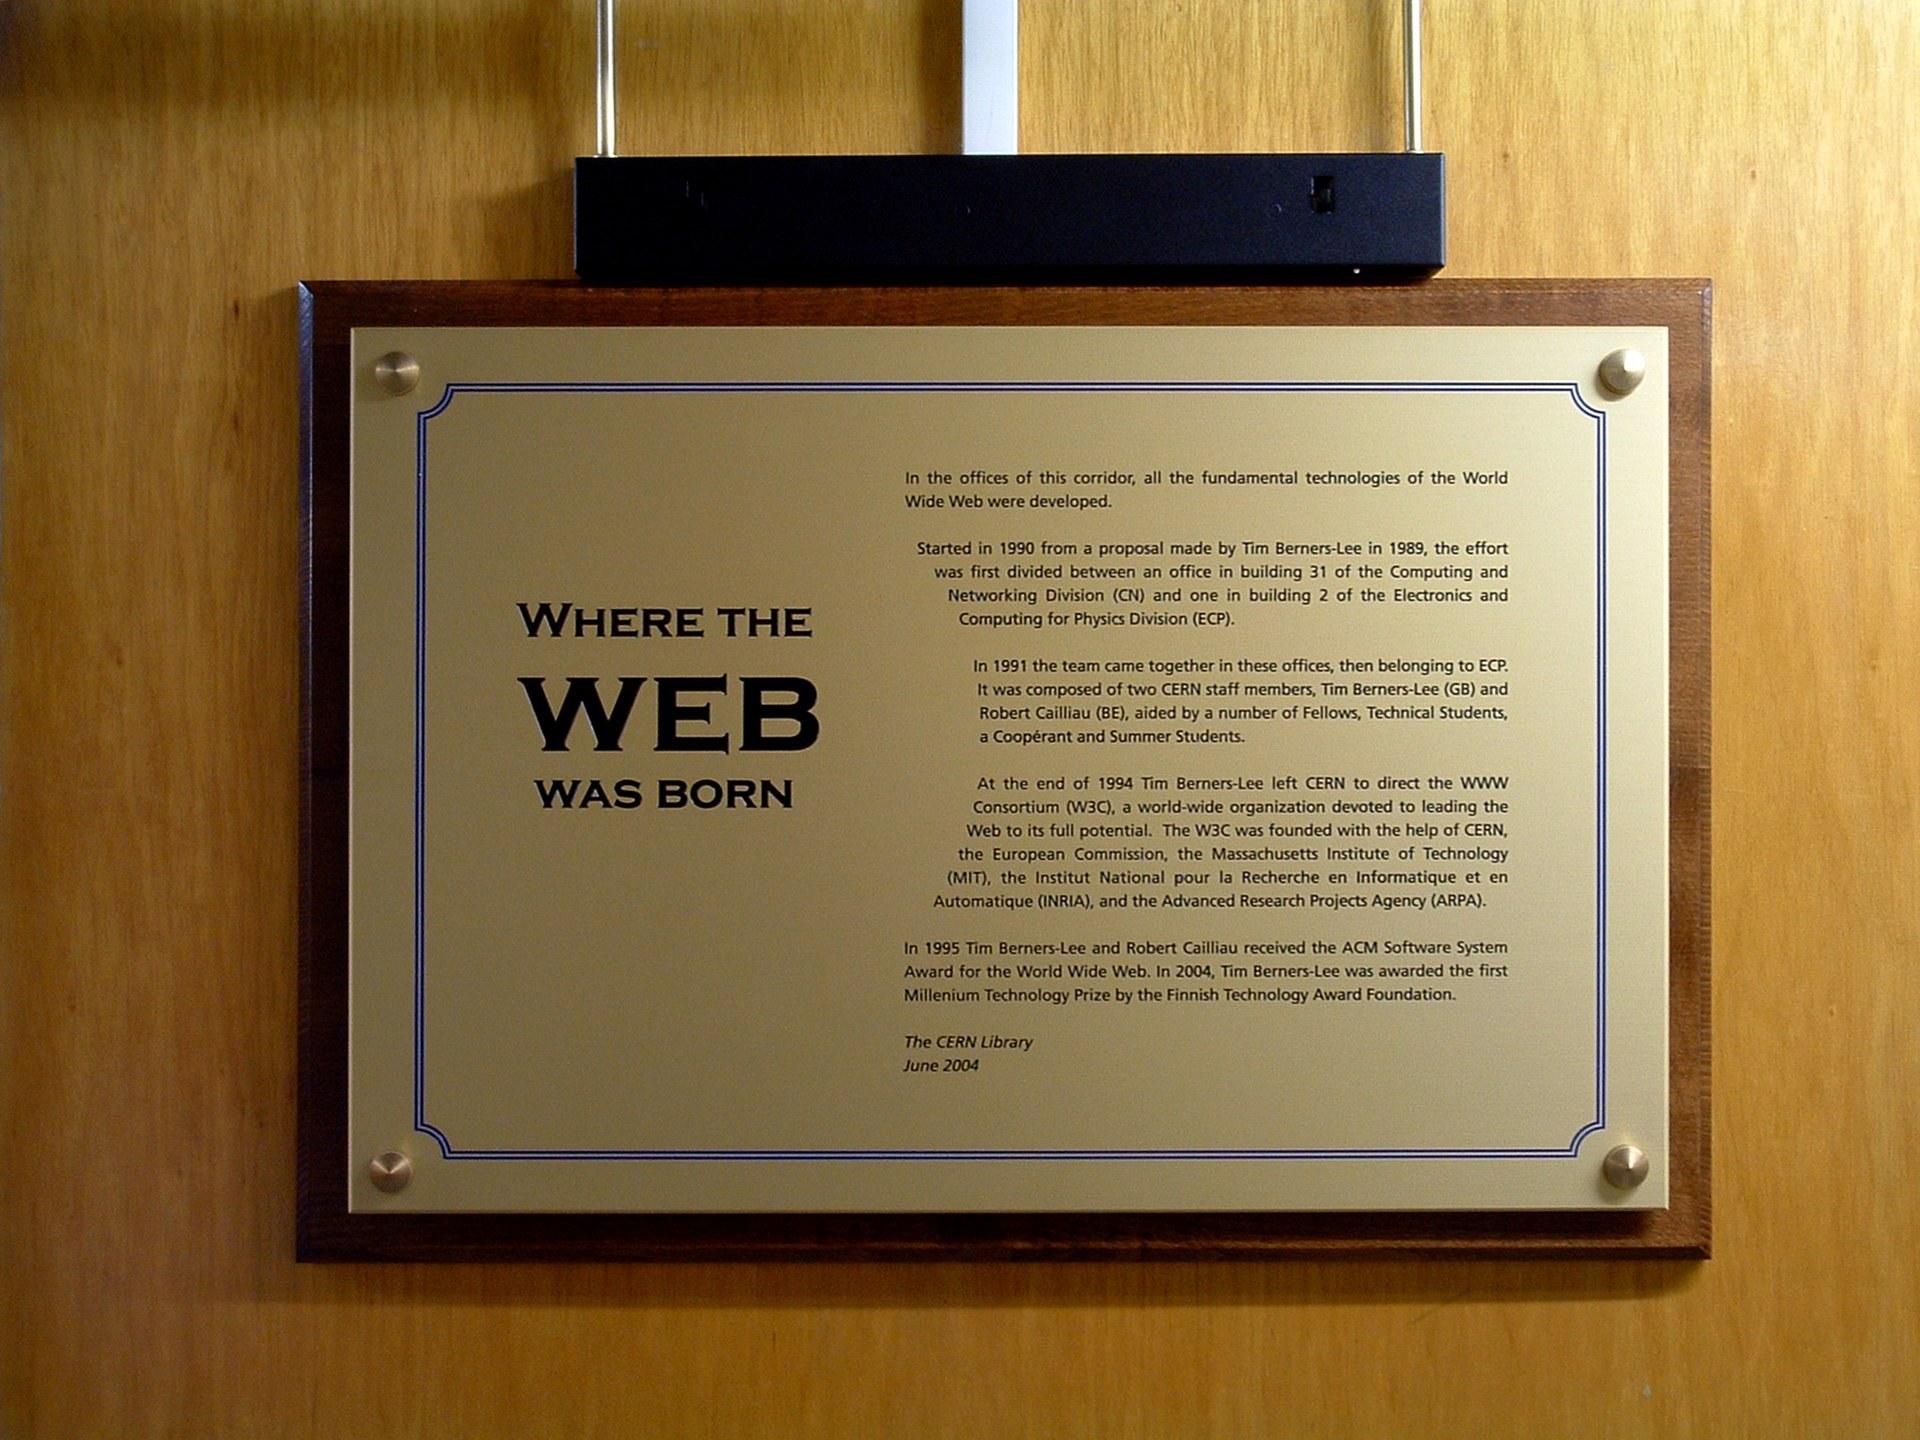
\includegraphics[width=\textwidth, center]{WEB.jpg}
            \caption{Plaque commémorative de l'invention du World Wide Web dans le bâtiment 1 du CERN}
            \label{WEB}
        \end{figure}

        Sur le LHC sont installés 4 principales expériences qui sont des collaborations internationales : ATLAS, CMS, ALICE et LHCb.
        Ces expériences prennent la forme de détecteurs. C'est à l'intérieur d'eux que se font les collisions dont les résidus sont détectés par plusieurs types de capteurs.

        La mise en oeuvre des expériences du CERN a depuis longtemps nécessité le développement de nouvelles technologies.
        Ainsi l'informatique et internet sont présent depuis longtemps afin de gérer la masse de données produites dans les détecteurs.
        Des programmes comportants plusieurs millions de lignes de codes sont exécutées aux centres de calcul sur les sites du CERN mais aussi partout autour du monde grâce au "Grid".
        Le CERN a aussi contribué au développement d'internet en Europe.

        \section{L'expérience LHCb}
        Le Large Hadron Collider beauty (Figure \ref{LHCb}) est l'une des 4 principales expériences installées sur le LHC.
        Elle vise l'étude du quark b afin de mesurer l'asymétrie entre matière et antimatière.
        La collaboration regroupe plus de 1200 personnes représentant plusieurs dizaines d'instituts.
        L'expérience se situe sur le point 8 du LHC.

        \begin{figure}[H]
            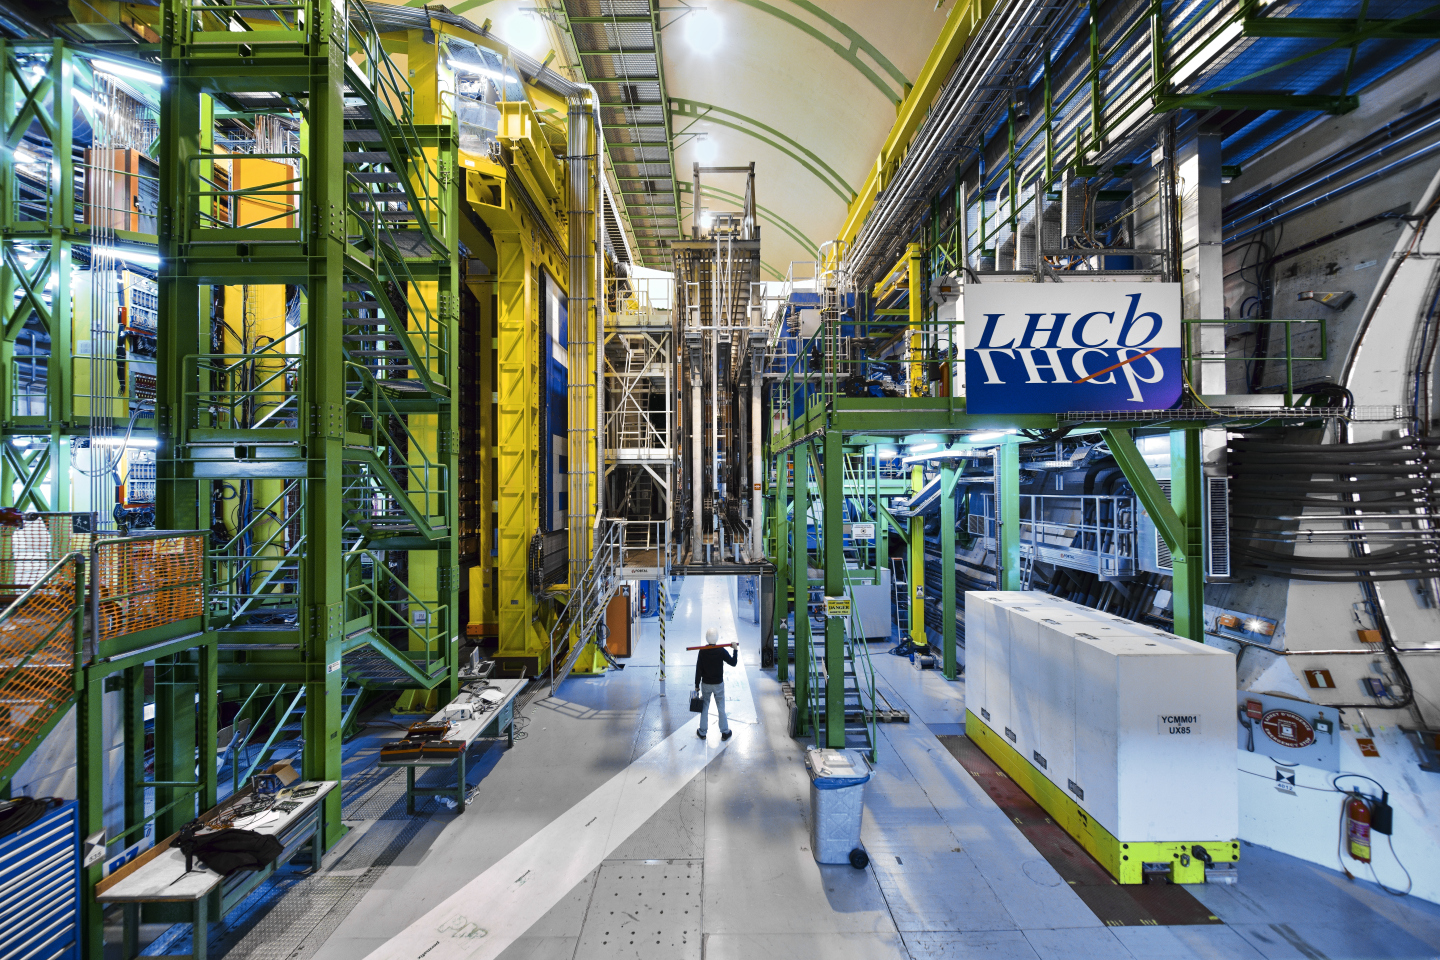
\includegraphics[width=\textwidth, center]{LHCb.jpg}
            \caption{LHCb}
            \label{LHCb}
        \end{figure}

        Le détecteur est composé de plusieurs instruments qui mesurent le passage des particules émises ors des collisions ainsi que certaines de leur propriétés.
        Grâce aux données recueillies, on peut reconstruire les trajectoires des particules ainsi que certaines de leur propriétés comme la masse ou la charge.

        \begin{figure}[!htb]
            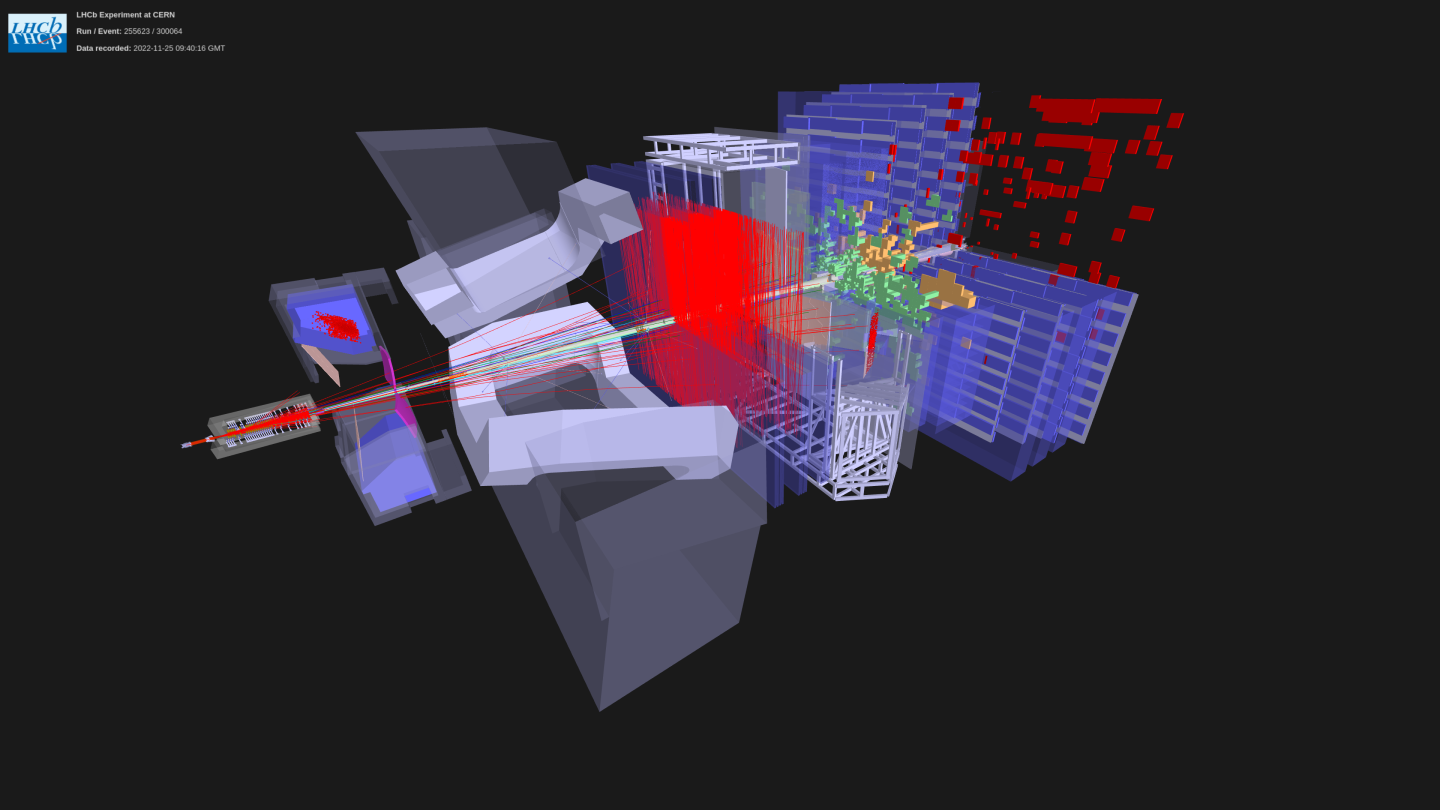
\includegraphics[width=\textwidth, center]{LHCb_3D.png}
            \caption{Modélisations de particules dans le détecteur}
            \label{LHCb_3D}
        \end{figure}

    \section{Computing Group}
        Les différents instruments du capteur produisent un flux de données conséquent d'environ $5 To$.
        Une importante infrastructure informatique est donc nécessaire pour pouvoir les traiter.

        \begin{figure}[!htb]
            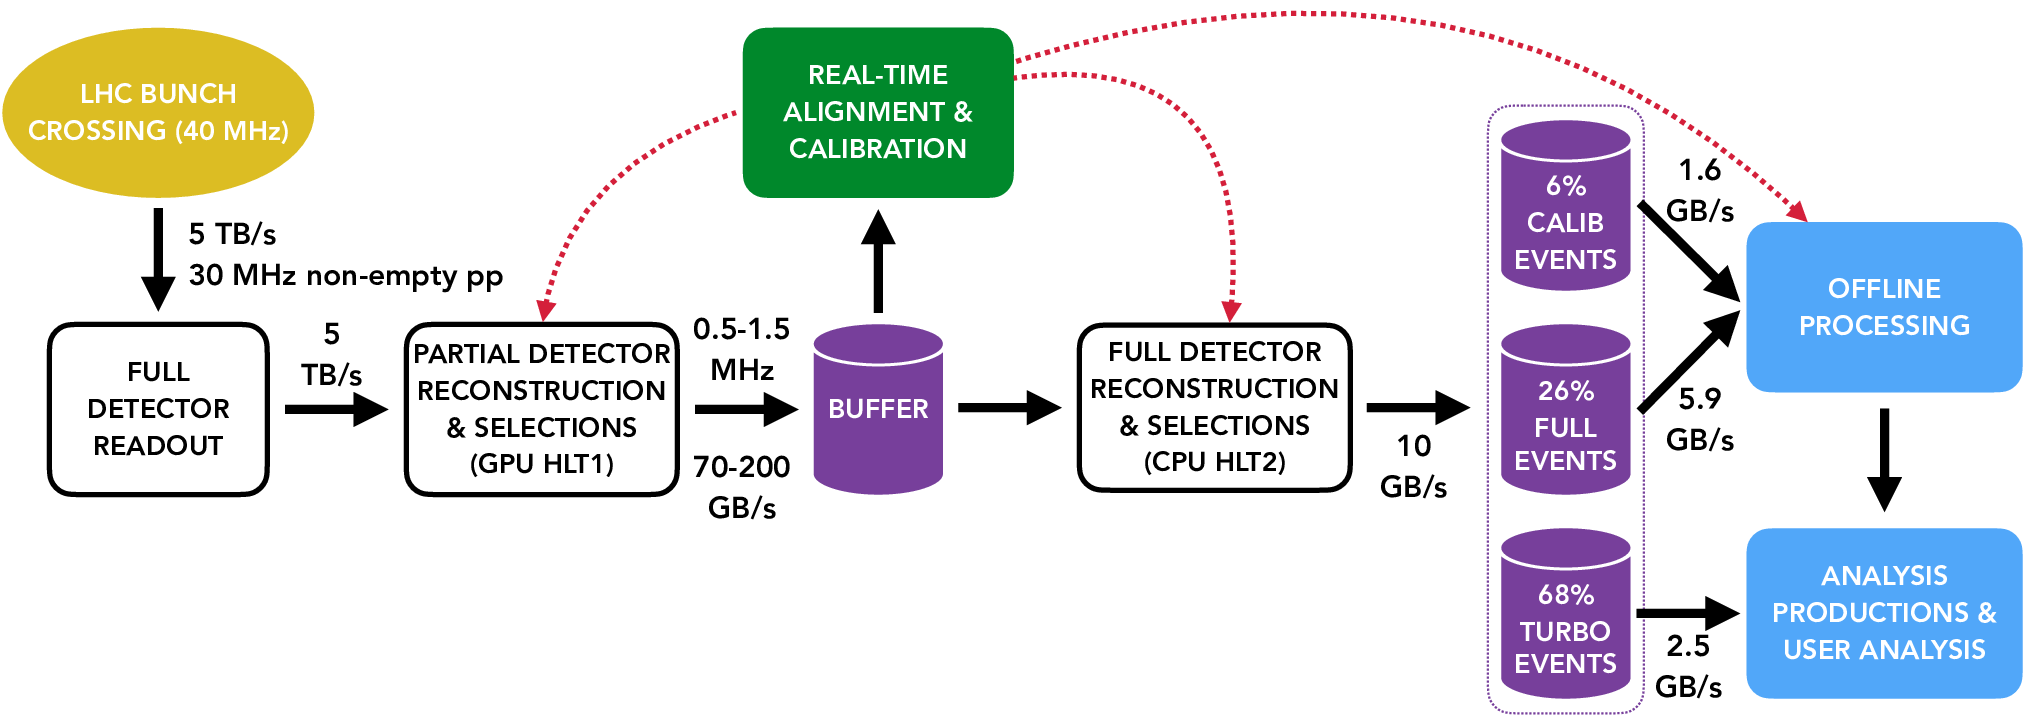
\includegraphics[width=\textwidth, center]{LHCb_stack.png}
            \caption{Infrastructure de gestion des données issues du détecteur}
            \label{LHCb_stack}
        \end{figure}

        LHCb utilise une pile de programmes (dont certains sont partagés avec d'autres expériences) qui traitent les données issues du détecteur.
        Cette pile contient plusieurs millions de lignes de codes.
        Ce code est principalement du C++ fait en grande partie par des physiciens non ingénieurs en informatique et dont certaines parties ont plusieurs décénies.

        Son maintient et son amélioration est donc un enjeux majeur.
        C'est le Computing Group du LHCb qui est chargée de cette tâche.

    \section{Travail à faire et analyse}
        Le code C++ de LHCb est compilé avec l'outil CMake qui permet de simplement définir les différentes cibles de compilation ainsi que leurs dépendances.
        Il est composé de plusieurs programmes qui forment une pile.
        On peut citer : Geant, Root, Gaudi qui sont partagés avec d'autres expériences et Detector, LHCb, Lbcom, Rec ou Moore qui sont spécifiquement pour LHCb.
        Tout ceci tourne sur des serveurs Linux et est largement \emph{multithreadé}

        L'objectif de ce stage est d'implémenter des solutions pour améliorer la rapidité de l'exécution du code.
        Les deux principales voies initialement envisagées sont l'utilisation de bibliothèques statiques à la place des dynamiques et la mise en place de profile-guided optimization.

    \section{Étude du problème}

        \subsection{Étapes de compilation}
            Un programme écrit dans un langage de programmation comme le C ou le C++ ne peut pas être exécuté directement.
            Pour ça, il doit d'abord être transformé en un fichier binaire exécutable par le système.
            On appelle ce processus la compilation.
            Le passage du code source au binaire final se fait en plusieurs étapes que voici :
            \begin{enumerate}
                \item Le \emph{préprocesseur} exécute les macros et les autres directives pour modifier le code source.
                \item Le \emph{compilateur} fait l'analyse lexicale et syntaxique pour produire du code assembleur à partir du code source.
                Il peut égallement faire des optimisations.
                C'est l'étape la plus importante.
                \item L'\emph{assemblage} du code assembleur en fichiers objets.
                Cette étape est souvent fusionnée avec la précédente.
                \item Le \emph{linker} fusionne les fichiers objets en un binaire.
                Pour cela il fait la résolution des différents symboles utilisés.
            \end{enumerate}

        \subsection{Types de bibliothèques}
            Il est possible de compiler du code C ou C++ non pas comme un exécutable mais comme une bibliothèque.
            Cette bibliothèque peut ensuite être linkée avec un exécutable ou une autre bibliothèque afin de lui fournir des fonctions ou symboles.
            Il existe plusieurs 3 types de bibliothèques.

            \subsubsection{STATIC}
                Une bibliothèque statique est une archive de fichiers objets.
                Lors du linkage avec un executable, ceux-ci sont simplement linkés avec les autres fichiers objets après la compilation.

            \subsubsection{SHARED}
                Une bibliothèque partagée est un fichier compilé sous forme de bibliothèque externe.
                On lui donne souvent l'extension \verb'.so' sous Linux ou \verb'.dll' sous Windows.
                Ce fichier n'est pas linké après la compilation mais au chargement de l'exécutable par le linker dynamique via une liste de dépendances que contient l'exécutable.

                Comme son nom l'indique, ce genre de bibliothèque peut être partagée par plusieurs binaires.
                Ainsi, si plusieurs exécutables utilisent la même bibliothèque partagée, il n'y a besoin de la compiler ou de la télécharger qu'une seule fois sur la machine.
                De plus, il est possible de mettre à jour la bibliothèque sans avoir besoin de mettre à jour les exécutables.

            \subsubsection{MODULE}
                Un module est en fait une bibliothèque partagée, à la différence qu'on la charge manuellement pendant l'exécution, alors qu'une bibliothèque partagée est automatiquement linkée au démarrage.
                Pour ce faire on utilise la fonction C \verb'dlopen' à laquelle on donne le chemin du module.

                Ainsi les modules permettent de charger complètement dynamiquement des parties de programme selon les besoins.
                Ils sont donc très utlisés dans LHCb afin de ne charger que ce qui est nécessaire pour éffectuer les calculs demandés.

                On peut aussi compiler et charger du code à la volée.
                Ce mécanisme est utilisé dans LHCb via ce qu'on appelle les foncteurs.

            \subsubsection{Cas de LHCb}
                La pile LHCb est découpée en centaines de petites parties.
                Ce découpage existe d'abord pour des raisons historiques car cela permettait de plus facilement collaborer sur le même projet avant l'arrivée de Git.
                Mais cela permet aussi de ne pas avoir à tout compiler et charger lorsqu'on a besoin que de travailler sur seulement certaines parties.

                De ce fait la pile une fois compilée se compose de centaines de bibliothèques et de modules dynamiques.
                Cette architecture est certes plus simple à utiliser mais il pourrait être intéressant d'étudier si leur fusion en un seul grand exécutable permettrait une meilleur performance en production.

        \subsection{Guided optimisation}
            Les compilateurs comme \emph{gcc} ou \emph{clang} possèdent des options qui permettent de compiler un programme mieux optimisé.
            Parmis ces optimisations on peut citer :
            \begin{itemize}
                \item l'\emph{inlining} qui est le fait de remplacer l'appel du'une fonction par le corps de la fonction elle-même ;
                \item la réorganisation des blocs, par exemple lorsqu'il y a un branchement ;
                \item la mise en registre de certaines variables.
            \end{itemize}
            Certaines de ces optimisations utlisent des heuristiques pour déterminer quelle possibilités est la plus probable.
            Tout ceci permet à un programme compilé en mode optimisé d'avoir une performance multpliée.

            Cependant les heuristiques utilisés sont quelques fois faux, ce qui représente un manque d'optimisation à gagner.
            Pour pouvoir faire mieux, il faudrait pouvoir savoir comment le programme se comporte en situation réelle afin de mieux choisir pour chaque cas quelle est la meilleure solution d'optimisation.

            \subsubsection{Profile-guided optimization}
                Le \emph{profile-guided optimization} est une technique qui conciste à :
                \begin{enumerate}
                    \item compiler une première fois le programme avec des options pour faire de l'instrumentation ;
                    \item faire tourner le programme de manière classique afin que l'instrumentation crée profiles sur le comportement du programme ;
                    \item recompiler le programme en utilisant les profiles précédemment créés pour mieux optimiser dans les détails.
                \end{enumerate}
                Cette technique permet souvent d'obtenir un gain de performance d'entre $5\%$ et $10\%$.

            \subsubsection{Feedback directed optimization}
                Cette solution proposée par Google repose sur le même principe que le PGO à la différence que la première compilation n'a pas besoin de se faire avec des options d'instrumentation.
                À la place, on utilise des outils de \emph{profiling} lors de l'exécution du programme pour créer les profiles.
                Cette technique peut être plus facile à mettre en oeuvre et offre des résultats sensiblement similaires.

            \subsubsection{Link-time optimization}
                Lorsqu'on compile un programme C ou C++, on compile indépendamment chaque fichier source (translation unit) en fichier objet.
                Ces fichiers sont ensuite réunis en un binaire par le \emph{linker}.
                De ce fait, le compilateur est incapable de faire des optimisations qui font intervenir plusieurs translation unit.
                Typiquement, le compilateur ne peut pas faire d'inlining si la définition de la fonction se trouve dans un autre fichier source.

                Le \emph{link-time optimization} permet d'éffectuer des optimisations supplémentaires au moment du \emph{link}.

        \subsection{Include-what-you-use}
            En C et en C++, on peut utiliser la directive préprocesseur \verb'#include' afin d'inclure un fichier \emph{header} qui contient des déclarations de classes et de fonctions.
            Le préprocesseur copie tout simplement le contenu du fichier inclu à l'endroit où la directive est appellée.
            Ce mécanisme est relativement simple mais peut poser des problèmes lorsque les programmes contiennent beaucoup de fichiers.

            En effet si un fichier \verb'C.cpp' inclus un fichier \verb'B.hpp' qui lui même inclus \verb'A.hpp', alors les symboles définis dans \verb'A.hpp' sont disponnibles dans \verb'C.cpp'.
            Si on les y utilise, alors on peut oublier d'inclure \verb'A.hpp' dans \verb'C.cpp'.
            En soit, cela n'est pas problématique, mais si plus tard on enlève \verb'A.hpp' de \verb'B.hpp' car on ne l'y utilise plus, alors on aura cassé la dépendance dans \verb'C.cpp'.

            Un autre problème encore plus grave serait d'avoir \verb'C.cpp' qui inclus d'abord \verb'A.hpp' puis \verb'B.hpp' mais que \verb'B.hpp' n'inclus pas \verb'A.hpp' alors qu'il utilise ses symboles.
            Ici on ne se rendrait pas compte qu'il manque une inclusion à cause du mécanisme de copier-coller.

            Pour tenter de résoudre ce genre de problèmes, il existe l'outil \emph{include-what-you-use} qui analyse le code de la même manière qu'un compilateur et qui signale et corrige les problème d'inclusions.
            Pour cela il suit la règle : un fichier header doit être inclus si et seulement si il existe au moins un symbole utilisé qui est défini dans ce header.

\chapter{Méthode}
    \section{Environnement de travail}
        Le travail s'est fait sur un serveur tournant sous \emph{CentOS 7}.
        Celui-ci possède 64 processeurs d'architecture \verb'x86_64' tourant à $3.7 MHz$ et formant 2 noeuds \emph{NUMA}.
        Le serveur possède de plus $187 Go$ de mémoire.

        L'infrastructure de LHCb est constituée d'une pile de programmes dont chaque couche dépend de celles précédentes.
        Classiquement, les programmes sont compilées un à un et indépendamment.
        Cependant cela est peu pratique lorsque l'on cherche à faire des optimisations sur l'ensmble des compilations.
        C'est pourquoi le travail a été éffectué sur une pile différente qui dispose d'un fichier \verb'CMakeLists.txt' global et qui s'applique donc à toute la pile.

        De plus, il est possible de compiler pour plusieurs platformes.
        Ici, il a été choisi de compiler vers \verb'x86_64_v3-centos7-gcc11+detdesc-opt+g'.
        En effet, au moment où le travail a été commencé, \verb'gcc11' était le compilateur avec lequel la pile était la plus stable.
        De plus, les machines les plus performantes ont une architecture \verb'x86_64_v3' et tournent sous \verb'centos7'.
        Enfin, il était pertinent d'utiliser une version déjà optimisée et avec les options de débuggage.

        Pour tester la rapiddité d'exécution des programmes, deux tests ont principalement été utilisés :
        \begin{enumerate}
            \item un test \emph{Hlt1} qui fait des analyses plus simples et dont les programmes sont déjà assez optimisés ;
            \item un test \emph{Hlt2} qui exécute des reconstructions bien plus poussées mais dont le code est de moins bonne qualité.
        \end{enumerate}

    \section{Diagrammes de Gantt}
        \begin{figure}[H]
            \begin{ganttchart}[
                expand chart=\linewidth,
                time slot format=little-endian,
            ]{01-04-2023}{31-08-2023}
                \gantttitlecalendar{month=name}\ganttnewline

                \ganttbar{Analyse}{01-04-2023}{31-04-2023}\ganttnewline
                \ganttbar{Bibliothèques statiques}{01-05-2023}{31-06-2023}\ganttnewline
                \ganttbar{PGO}{01-07-2023}{31-08-2023}
            \end{ganttchart}
            \caption{Diagramme de Gantt prévisionnel.}
            \label{Gantt_previsionnel}
        \end{figure}

        \begin{figure}[H]
            \begin{ganttchart}[
                expand chart=\linewidth,
                time slot format=little-endian,
            ]{01-04-2023}{31-08-2023}
                \gantttitlecalendar{month=name}\ganttnewline

                \ganttbar{Analyse}{01-04-2023}{10-04-2023}\ganttnewline
                \ganttbar{Bibliothèques statiques}{11-04-2023}{15-05-2023}\ganttnewline
                \ganttbar{PGO}{01-05-2023}{31-05-2023}\ganttnewline
                \ganttbar{Include-what-you-use}{29-05-2023}{11-06-2023}\ganttnewline
                \ganttbar{Fast-math}{12-06-2023}{31-06-2023}
            \end{ganttchart}
            \caption{Diagramme de Gantt.}
            \label{Gantt}
        \end{figure}

    \section{Fusion des bibliothèques dynamiques}

        \subsection{Graphe des dépendances}
            Déjà, une première chose est d'avoir une idée des dépendances entre bibliothèques.
            Pour cela, un outil intégré à CMake permet de créer des graphes des dépendances.
            Pour cela, il suffit d'ajouter un argument lors de la configuration de CMake :
            \begin{verbatim}
--graphviz=path/to/files.dot
            \end{verbatim}

            On peut ensuite convertir les graphes produits en images :
            \begin{verbatim}
dot -Tsvg -o path/to/file.svg path/to/file.dot
            \end{verbatim}

            Il peut être utile de cacher les bibliothèques externes car elles ne dépendent pas de nous :
            \begin{verbatim}
GRAPHVIZ_EXTERNAL_LIBS=FALSE
            \end{verbatim}

        \subsection{Passage des bibliothèques partagées en biliothèques statiques}
            Intéressous-nous à remplacer les bibliothèques partagées par des bibliothèques statiques.

            C'est le code CMake qui compile le code, crée les bibliothèques et les link.
            Ainsi, dans le programme Gaudi, il y a déjà des fonctions CMake qui permettent de facilement créer des bibliothèques partagées, \verb'gaudi_add_library', et des modules, \verb'gaudi_add_module'.
            Il est donc simple de copier la fonction \verb'gaudi_add_library', qui crée une bibliothèque partagée, en une fonction \verb'gaudi_add_static_library'.
            Cette fonction utilise la fonction CMake \verb'add_library' dans laquelle il suffit de changer le paramètre \verb'STATIC' en \verb'SHARED'.

            Avec cette nouvelle fonction, il est désormais facile de remplacer les bibliothèques partagée de la pile LHCb en bibliothèques statiques.

            Cependant, à cette étape là, on peut se retrouver dans un cas où une bibliothèque statique est linkée (et donc intégrée) à une bibliothèque dynamique ou à un module.
            Or le principe d'une bibliothèque dynamique est que comme elle est chargée dynamiquement, elle peut se retrouver à plusieurs endroits dans la mémoire, elle doit donc être compilée en \emph{position-independant code} pour pouvoir fonctionner.
            Ce n'est pas le cas d'une bibliothèque statique pour laquelle on sait à la compilation où son code machine sera en mémoire.
            On doit rajouter l'option de compilation \verb'-fpic' pour compiler les bibliothèques statiques en position-independant code (on pourra l'enlever lorsque tout sera statique).

        \subsection{Passage des modules en bibliothèques statiques}
            Cherchons maintenant à rendre les modules statiques.

            Gaudi propose égallement une fonction CMake \verb'gaudi_add_module'.
            On peut donc simplement remplacer les appels à cette fonction par l'appel à la fonction précédemment créée \verb'gaudi_add_static_library'.
            Il faut égallement linker ces nouvelles bibliothèques statiques avec l'exécutable.
            Pour cela il suffit d'utiliser la fonction CMake \verb'target_link_libraries' sur l'exécutable.

            Ceci compile, en revanche il y a un problème à l'exécution.
            En effet par défaut le linker supprime le code qui n'est pas utilisé.
            Or jusqu'à présent, chaque module comprenait une partie qui était exécutée à son chargement et qui enregistrait le module dans une table.
            En statique, cette fonction n'est donc pas utilisée et est donc supprimée.
            De ce fait l'exécutable ne sait pas que le module est déjà chargé.

            Résoudre ce problème correctement consisterait à revoir en profondeur ce système, ce qui semble trop complexe à ce stade.
            La solution retenue a été d'utiliser l'option de linkage \verb'-Wl,--whole-archive' qui force le linker à garder l'ensemble du code.
            Cependant avec cela des symboles sont inclus plusieurs fois ce qui mène à une erreur que l'on peut désactiver avec \verb'-Wl,--allow-multiple-definition'.
            Il n'est normallement pas recommandé d'utiliser ses options car elles ne correspondent pas au comportement usuel du linker et peuvent donc être à l'origine de bugs ou de mauvaises optimisations.

            Un autre problème est que l'on charge toujours dynamiquement quelques modules, notamment des foncteurs.
            Or ceci ont besoin des symboles définis dans les bibliothèques désormais statiques qui ne sont donc plus visibles.
            Il faut donc activer l'option \verb'-Wl,--export-dynamic' pour résoudre cet autre problème.


    \section{Guided optimization}

        \subsection{Profile-guided optimization}
            \subsubsection{Mise en place}
                Le profile-guided optimization est inclus dans gcc et dans clang.
                Pour cela il faut utiliser le flag de compilation \verb'-fprofile-generate' qui va permettre de compiler une version du programme avec instrumentation.

                Ainsi, lorsqu'on va faire tourner le programme, des fichiers de profiles vont être générés, ils correspondent à des compteurs qui permettent de connaitre l'utilisation de chaque fonction et branchement.

                Ensuite pour compiler le programme final, il faut utiliser le flag \verb'-fprofile-use' pour utiliser les profiles.
                On peut aussi rajouter le flag \verb'-fprofile-correction' pour corriger certains problèmes qui peuvent apparaître avec le \emph{multi-threading}.

                Ces flags sont mis de manière globale sur l'ensemble du projet CMake.

            \subsubsection{Difficultés}
                Le profile-guided optimization n'a d'abord pas donné de résultats, la vitesse d'exécution ne changeant pas.
                C'est après un certain temps que l'on a compris que le PGO n'est éfficace que si le link-time optimization est égallement activé.

        \subsection{AutoFDO}
            Même si le principe général est similaire, la mise en place de AutoFDO diffère du PGO.

            Tout d'abord la première compilation se fait normallement.

            C'est ensuite lorsqu'on exécute le programme qu'on doit le faire en utilisant un outil de profiling.
            Le plus simple à utiliser sous Linux est \verb'perf'.
            \begin{verbatim}
perf record -b -e -- run_command
            \end{verbatim}
            Il faut ensuite convertir les fichiers :
            \begin{verbatim}
create_gcov --binary=path/to/binary -- profile=perf.data --gcov=perf.gcov -gcov_version=1
            \end{verbatim}

            Enfin on recompile l'exécutable avec le flag \verb'-fauto-profile=perf.gcov'.

        \subsection{Link time optimization}
            La mise en place du link-time optimization se fait à deux moments différents.
            Tout d'abord au moment de la compilation des fichiers source en fichiers objets.
            Puis au moment du link.
            Avec gcc, cela se fait dans les deux cas via le flag \verb'-flto'.

            Cependant dans CMake, il y a une meilleure manière de faire :
            \begin{verbatim}
include(CheckIPOSupported)
check_ipo_supported()
set(CMAKE_INTERPROCEDURAL_OPTIMIZATION TRUE)
            \end{verbatim}
            Ici, on commence par vérifier que l'\emph{interprocedural optimization} (synonyme de \emph{link-time optimization}) est supportée, puis on l'active de manière globale.
            Cette solution a l'avantage de laisser CMake mettre en place le LTO pour la compilation et le link.

            On peut remarquer que ceci augmente encore plus le temps de construction des programmes (environ $50\%$).

        \subsection{VTune}
            L'outil VTune créé par \emph{Intel} permet de comprendre l'utilisation du processeur par un programme.
            On peut notamment voir le taux de mauvaises prédictions de branchement ou le temps que le processeur passe à attendre la mémoire.

            \begin{figure}[H]
                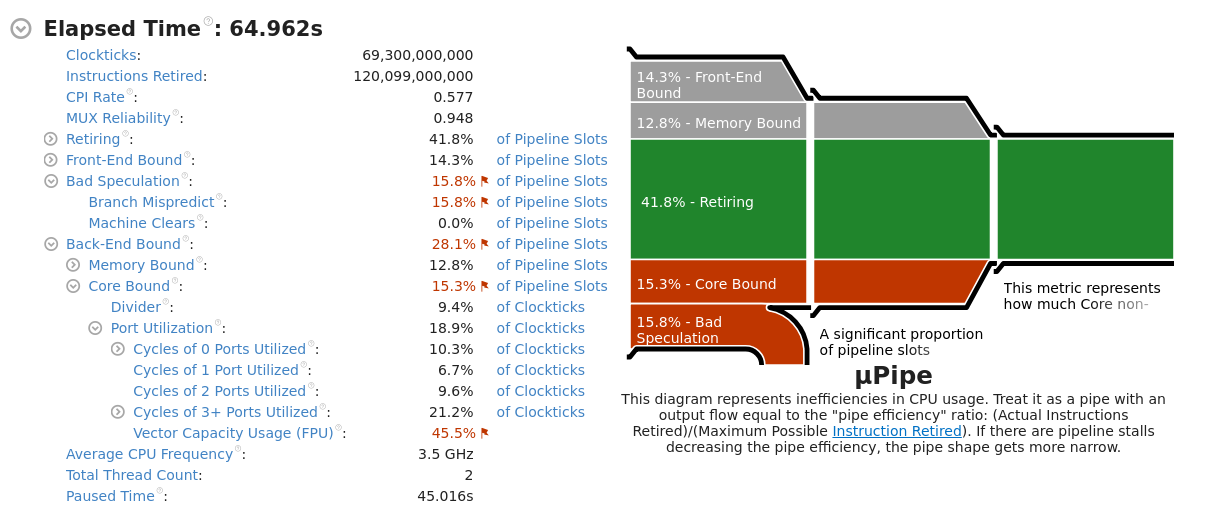
\includegraphics[width=\textwidth, center]{vtune_hlt1.png}
                \caption{Résumé de VTune pour le test \emph{Hlt1}}
                \label{vtune_hlt1}
            \end{figure}

            \begin{figure}[H]
                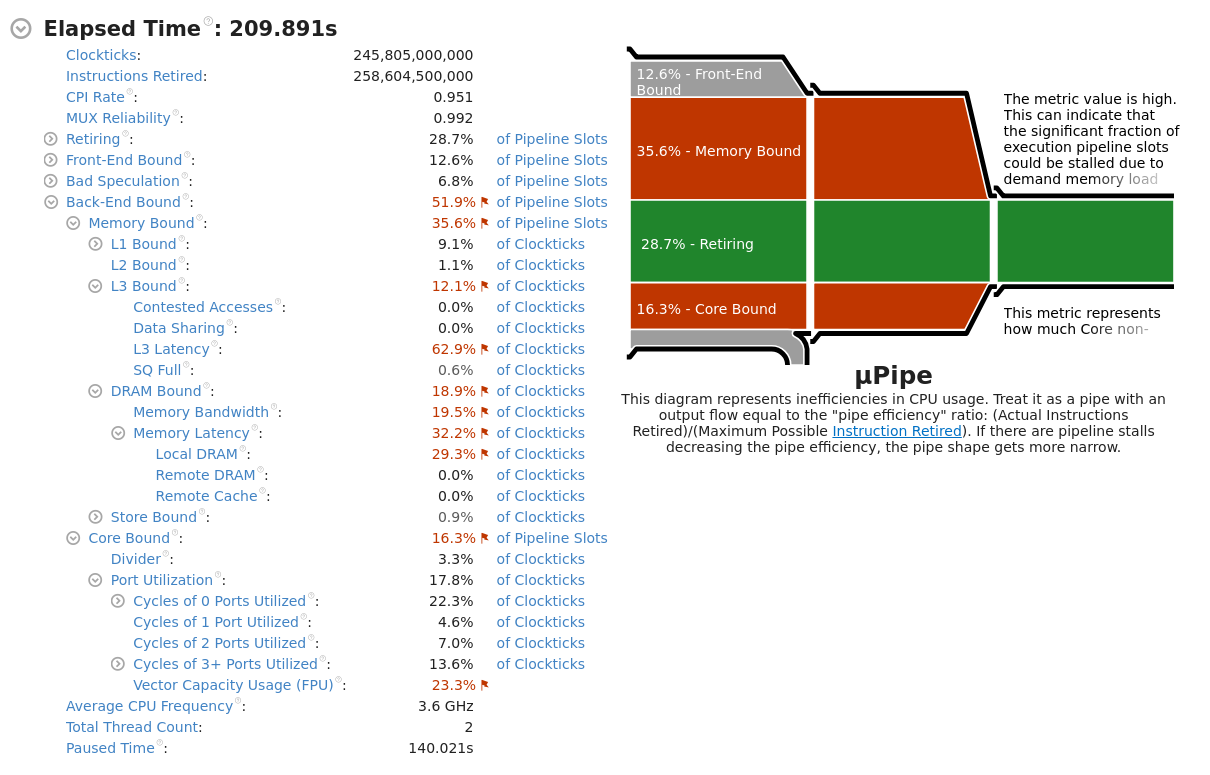
\includegraphics[width=\textwidth, center]{vtune_hlt2.png}
                \caption{Résumé de VTune pour le test \emph{Hlt2}}
                \label{vtune_hlt2}
            \end{figure}

            On peut remarquer que le test \emph{Hlt1} optimise de base beaucoup mieux l'utilisation du processeur que le test \emph{Hlt2}.

    \section{Include-what-you-use}
        \emph{iwyu} a été conçu pour fonctionner avec \emph{clang} et \emph{llvm}.
        Encore une fois, il est aisé d'utiliser cet outil à travers CMake.
        En effet il suffit de donner à la variable \verb'CMAKE_CXX_INCLUDE_WHAT_YOU_USE' la commande faisant tourner \verb'include-what-you-use'.
        Il faut alors faire tourner CMake avec la version de \emph{clang} correspondante comme compilateur.

        Il y avait une version du programme compatible avec \verb'clang12' installé sur le système.
        Cependant, il y a rapidemment eu un bug, l'outil gérant mal certaines références cycliques.
        Après recherche, ce bug n'a été corrigé qu'avec la dernière version de \emph{iwyu}, qu'il a donc fallut télécharger et recompiler avec \verb'clang16'.

        L'outil a alors correctement pu tourner.
        En revanche on a alors remarqué qu'il y avait toujours des bugs, notamment il supprimait parfois des inclusions en faite nécessaire ou en rajoutait qui ne servaient pas directement.
        De plus, on a pu se rendre compte que certaines architecture utilisés, comme les fichiers contenant le code de \emph{templates}, étaient incompatibles avec le principe de l'outil.

        Finallement, la mise en place de \emph{include-what-you-use} a été abandonnée et n'a servi qu'à repérer et corriger quelques erreurs déjà présentes.

\chapter{Résultats}

    \section{Amélioration de la rapidité d'exécution}
        Pour mesurer les améliorations, des \emph{throughput test} ont été faits.
        Aucun résultat n'a été observé avec le test \emph{Hlt1}, voici ceux de \emph{Hlt2} :

        \begin{center}
            \begin{tabular}{ c c c }
                Optimisation & Amélioration & Intervalle de confiance ($2\sigma$) \\
                LTO & $0.17\%$ & $\pm 1.12\%$ \\
                LTO \& PGO & $6.74\%$ & $\pm 1.44\%$ \\
                Static LTO & $0.87\%$ & $\pm 0.60\%$ \\
                Static LTO \& PGO & $6.88\%$ & $\pm 0.83\%$
            \end{tabular}
        \end{center}

    \section{Bibliothèques statiques}
        L'exécutable final passe de $\sim 20 Ko$ à $2,5 Go$.

        On remarque qu'utiliser des bibliothèques statiques à la place des dynamiques ne change pas significativement la rapidité.
        En revanche on a bien vu que cela pouvait entraîner des bugs supplémentaires, notamment avec les foncteurs.

    \section{Guided optimization}
        \subsection{Gain}
            Il y a un net gain de performance à utiliser le \emph{profile-guided optimization} et le \emph{link-time optimization} (environ $7\%$ d'amélioration).
            Ceci peut représenter plusieurs millers de machines à l'échelle des centres de calculs du LHCb.

        \subsection{Code final}
            Le code finallement ajouté au CMake global du projet est :
            \begin{lstlisting}[language=make,breaklines=true,numbers=left]
if("${PGO}" MATCHES "GENERATE")
    message("PGO generate")
    set(CMAKE_CXX_FLAGS "${CMAKE_CXX_FLAGS} -fprofile-generate")
endif()
if("${PGO}" MATCHES "USE")
    message("PGO use")
    set(CMAKE_CXX_FLAGS "${CMAKE_CXX_FLAGS} -fprofile-use -fprofile-correction")
endif()
include(CheckIPOSupported)
check_ipo_supported()
set(CMAKE_INTERPROCEDURAL_OPTIMIZATION TRUE)
            \end{lstlisting}

        \subsection{Mise en production}
            En l'état il n'est pas évident de mettre en production une version PGO.
            En effet les programmes sont pour l'instant compilés et installés un à un.
            Or le PGO nécessite de tout compiler une fois pour pouvoir faire tourner le programme.
            Il faudrait donc changer la manière d'installer les programmes pour utiliser plus simplement cette version.

\chapter*{Conclusion}


\printbibliography

\end{document}
